% 第 6 章 数据全链路与台账管理
\chapter{数据全链路与台账管理}

\section{数据流转全景}

\begin{figure}[htbp]
  \centering
  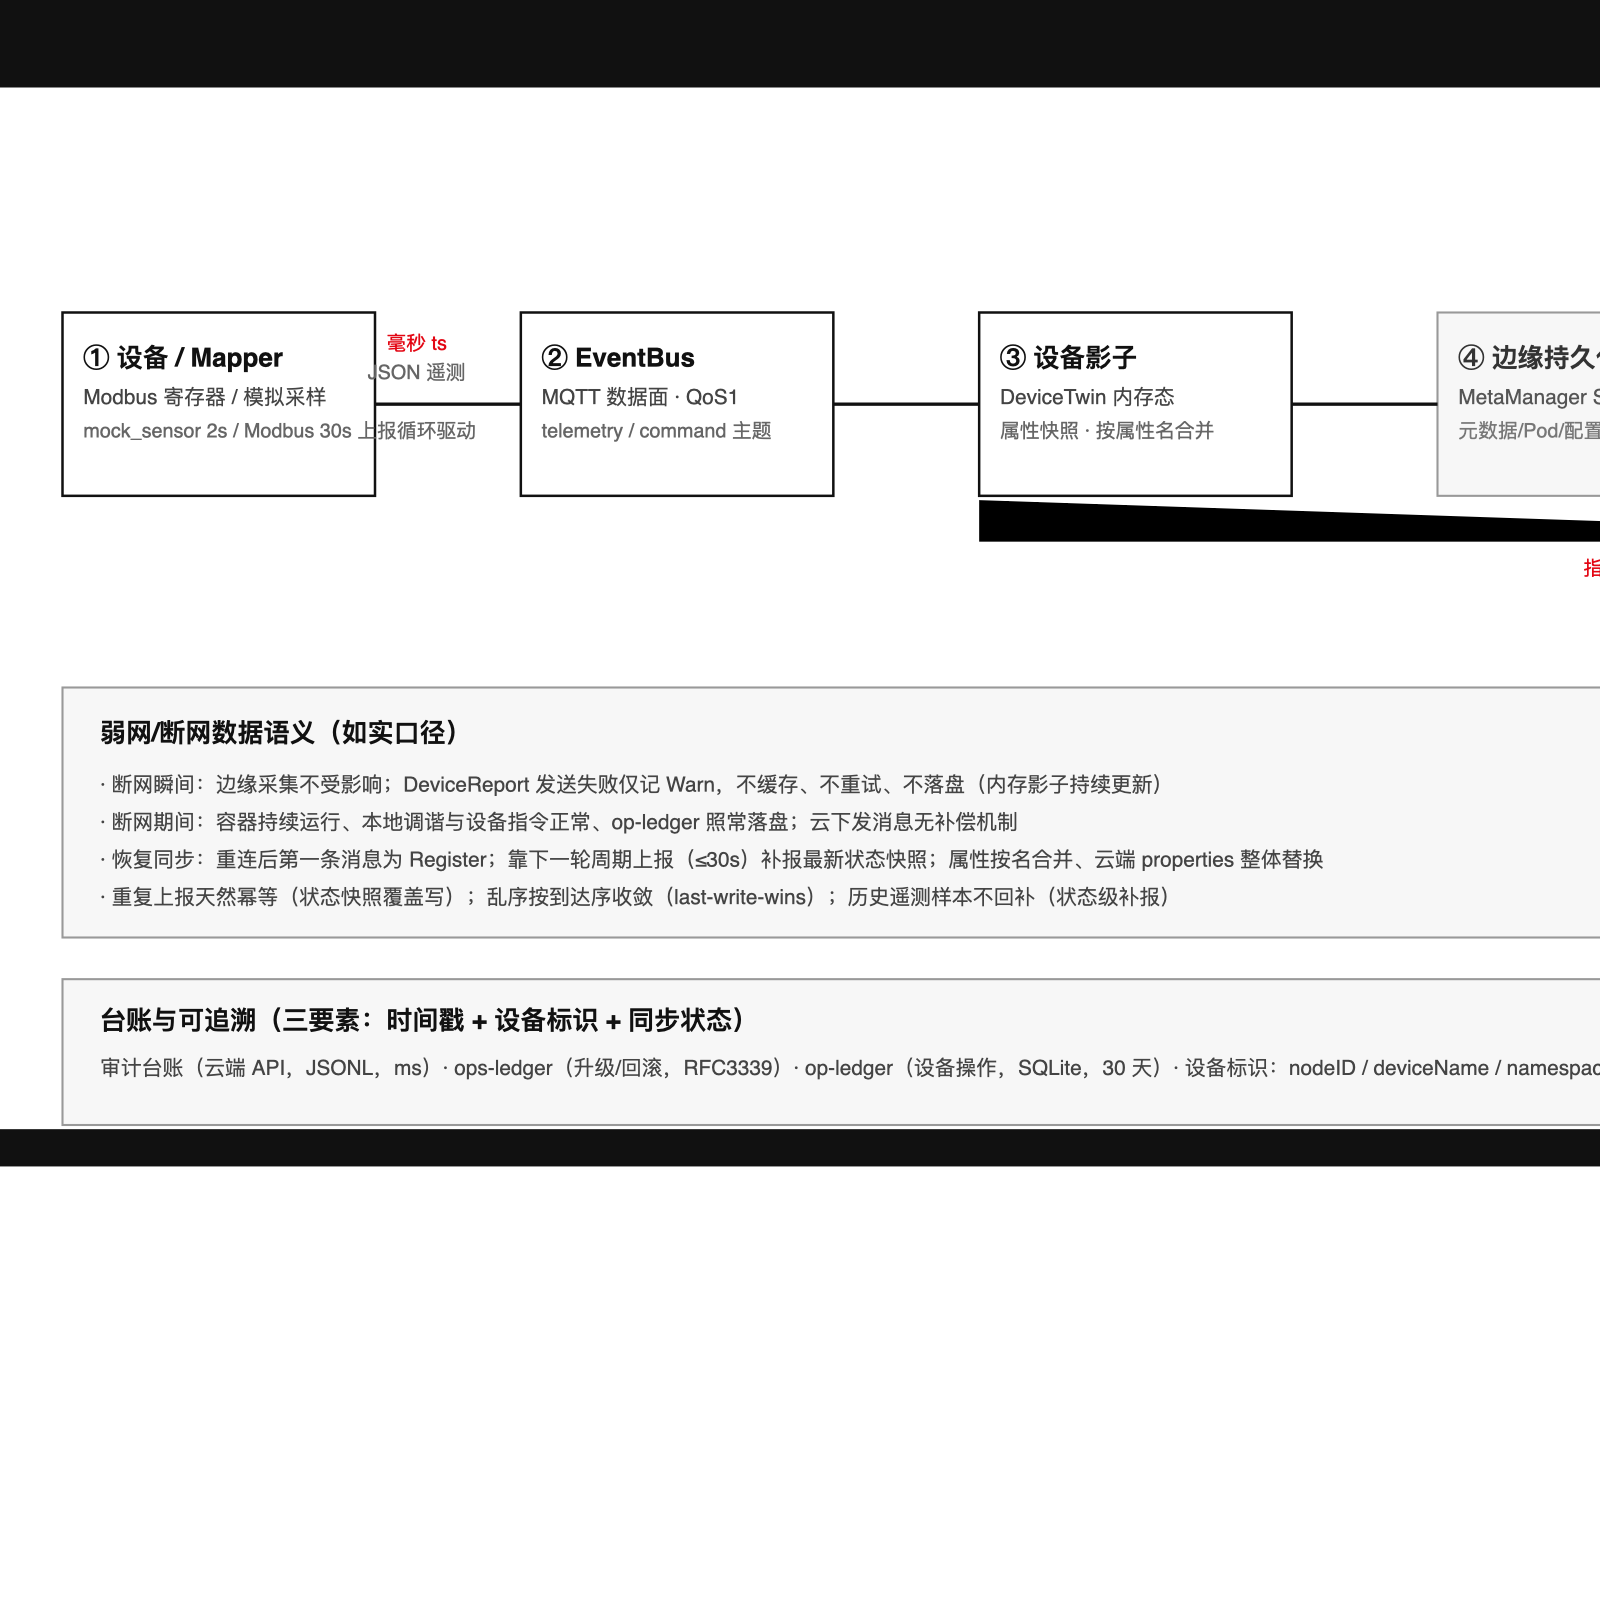
\includegraphics[width=0.94\textwidth]{../diagrams/dataflow.png}
  \caption{EdgeFlow 数据全链路}
  \label{fig:dataflow}
\end{figure}

\textbf{表 6-1：遥测数据上行 7 跳链路}

{\small\setlength{\tabcolsep}{3pt}
\begin{tabular}{@{}p{0.7cm}p{2.2cm}p{3.6cm}p{4.0cm}p{4.2cm}@{}}
\toprule
跳次 & 环节 & 数据内容 & 通道/协议 & 关键参数\\
\midrule
1 & 设备 $\rightarrow$ Mapper & 原始遥测 & Modbus TCP（读保持寄存器）/ mock\_sensor 内存波动 & Modbus 由 30s 上报循环驱动；mock\_sensor 2s 波动\\
2 & Mapper $\rightarrow$ EventBus & JSON 遥测 \{temperature, humidity, ts(毫秒)\} & MQTT QoS1；主题 \seqsplit{\texttt{devices/<namespace>/<device>/telemetry}}，指令订阅 .../command & QoS1 至少一次投递\\
3 & Mapper $\rightarrow$ 设备影子 & 属性快照 & DeviceTwin 内存态写入 & 影子仅维护最新快照\\
4 & 影子 $\rightarrow$ 边缘存储 & 节点元数据、Pod 期望状态、配置 & MetaManager SQLite（WAL） & 影子本身不落盘\\
5 & 影子 $\rightarrow$ 云端 DeviceReport & 设备状态报告 & WebSocket JSON，无 Ack 单向流式 & 30s 周期；\env{EDGEFLOW\_EDGECORE\_DEVICE\_REPORT\_INTERVAL} 可配（1s--10min）；启动即报一轮\\
6 & 云端接收 $\rightarrow$ 存储 & DeviceStatus 快照 & CloudCore 内存态 & nodeID $\rightarrow$ namespace/deviceName $\rightarrow$ 状态\\
7 & 云端存储 $\rightarrow$ API & 设备状态查询 & REST API & \seqsplit{\texttt{GET /api/v1/devices}}；\seqsplit{\texttt{GET /api/v1/nodes/\{nodeID\}/devices}}\\
\bottomrule
\end{tabular}}

\textbf{指令下行链路}：\seqsplit{\texttt{POST /api/v1/nodes/\{nodeID\}/device-command}} $\rightarrow$ 可靠投递（5s 超时、最多 3 次尝试、同一命令 ID 重发、边缘幂等去重 1000 条，F05）$\rightarrow$ Mapper 执行 $\rightarrow$ 写入 Twin.Desired $\rightarrow$ 云端合并状态。

\section{弱网下的数据语义}

EdgeFlow v0.1.0 的弱网数据语义为\textbf{“最新状态快照周期补报”}，如实说明如下：

\begin{itemize}
  \item \textbf{上行采集不依赖云边通道}：设备 $\rightarrow$ Mapper $\rightarrow$ EventBus $\rightarrow$ 设备影子的链路完全在边缘本地完成，云边通道中断不影响边缘采集与影子更新；
  \item \textbf{云端视角}：云端 DeviceStatus 为最新状态快照（内存态）。云边断连期间，云端展示的是最后一次成功收到的 DeviceReport；连接恢复后，边缘按 30s 周期（可配 1s--10min）补报最新快照，且每次边缘启动即上报一轮；
  \item \textbf{不做历史回补}：平台不提供历史数据断点续传与回补（断网期间样本不落盘，仅做状态级补报）。若业务需要历史遥测留存，需在 EventBus 侧或应用侧自行订阅持久化（v0.1.0 未内置遥测历史存储）；
  \item \textbf{下行指令弱网保障}：依赖可靠投递机制（5s 超时、最多 3 次尝试、同 ID 重发、边缘幂等去重 1000 条，F05），通道恢复后重发指令仍可正确投递且不重复执行，降低弱网下指令丢失/重复的风险。
\end{itemize}

\section{台账与可追溯}

\textbf{表 6-2：三类台账}

{\small\setlength{\tabcolsep}{4pt}
\begin{tabular}{@{}p{1.5cm}p{2.6cm}p{3.4cm}p{2.8cm}p{5.0cm}@{}}
\toprule
台账 & 记录内容 & 存储位置 & 格式与保留 & 关键字段\\
\midrule
审计台账 & 云端 API 操作（含 401 拒绝） & 默认 data/audit-ledger.jsonl（env \env{EDGEFLOW\_CLOUDCORE\_AUDIT\_PATH} 可配） & JSONL 追加；文件 0600 / 目录 0700 & ts(毫秒) / action / path / method / status / operator(默认 anonymous) / ip\\
ops-ledger & keadm 升级/回滚操作 & output-dir/ops-ledger.jsonl & JSONL 追加；keadm ops-ledger 查询最近 N 条（默认 20） & ts(RFC3339) / action(upgrade|rollback) / from / to / result(ok|failed) / operator(KEADM\_OPERATOR，缺省 unknown) / note(备份 id、失败原因)\\
op-ledger & 设备操作流水（采集/下发） & SQLite 追加流水 & 30 天保留 & id 自增 / ts 毫秒 / deviceId / direction(up 采集、down 下发) / regAddr / value / result(ok|error) / message\\
\bottomrule
\end{tabular}}

\textbf{时间戳与设备标识口径（表 6-3）}

\begin{tabular}{ll}
\toprule
口径项 & 约定\\
\midrule
时间戳 & 审计台账与 op-ledger 采用毫秒；ops-ledger 采用 RFC3339\\
节点标识 & nodeID，默认 edge-\texttt{<主机名>}\\
设备标识 & deviceName（如 sensor-01、mb-sensor-01）\\
命名空间 & namespace，默认 default\\
\bottomrule
\end{tabular}

\begin{quote}
跨台账关联时须按上述统一口径对齐，避免口径混用导致追溯断链。
\end{quote}

\section{数据可追溯记录要求}

可追溯性由\textbf{三个要素}构成，任一可追溯记录须同时满足：

\begin{enumerate}
  \item \textbf{时间戳}：标识“何时发生”——审计/设备操作为毫秒，系统变更为 RFC3339；
  \item \textbf{设备标识}：nodeID + deviceName + namespace 三元组，标识“发生在哪个节点、哪台设备”；
  \item \textbf{同步状态}：result/status 字段（ok/error/failed、up/down、HTTP 状态码），标识“结果如何、处于何种状态”。
\end{enumerate}

三类台账协同形成可追踪闭环：\textbf{审计台账}覆盖云端 API 操作（含 401 拒绝记录），\textbf{ops-ledger} 覆盖系统升级/回滚变更（含备份 id 与失败原因），\textbf{op-ledger} 覆盖设备级采集/下发流水（30 天保留）。结合 6.3 的统一口径，可对“谁在什么时间、通过什么操作、影响了哪台设备、结果如何”进行完整追溯。
